\begin{figure*}[t]
    \centering
    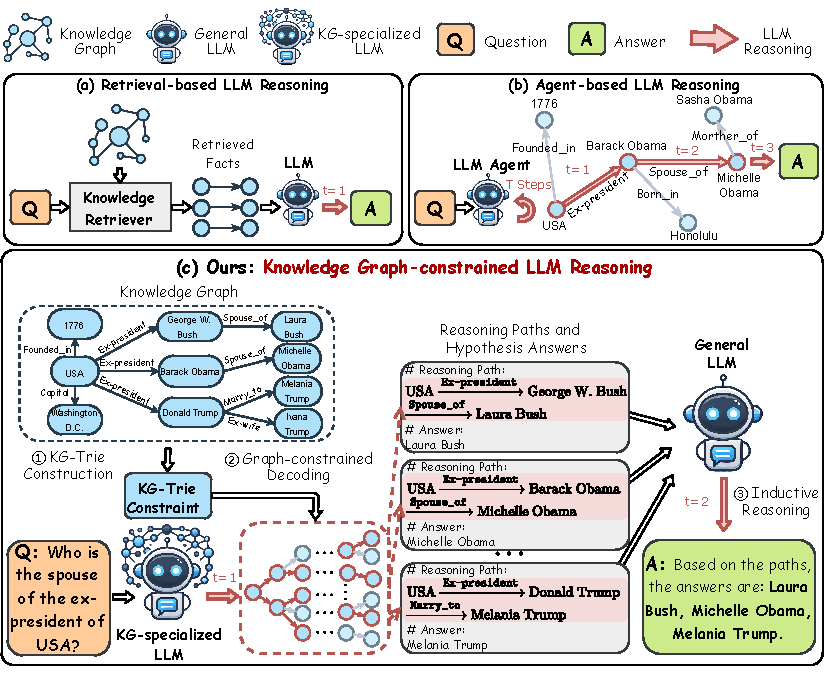
\includegraphics[width=.84\textwidth]{images/framework.pdf}
    \vspace{-.6cm}
    \caption{Illustration of existing KG-enhanced LLM reasoning paradigms and proposed graph-constrained reasoning (\ourmethod), which consists of three main components: 1) Knowledge Graph Trie Construction: building a structural index of KG to guide LLM reasoning, 2) Graph-constrained Decoding: generating KG-grounded paths and hypothesis answers using LLMs, and 3) Graph Inductive Reasoning: reasoning over multiple paths and hypotheses to derive final answers.}
    \label{fig:framework}
    \vspace{-0.5cm}
\end{figure*}



% 1) First, given a KG, we convert it into the KG-Trie, serving as a structured index to facilitate efficient reasoning path searches using LLMs. 2) Then, we design a graph-constrained decoding process that employs a lightweight KG-specialized LLM to generate multiple KG-grounded reasoning paths and hypothesis answers. This ensures the faithfulness of the reasoning process while leveraging the strong capabilities of LLMs to efficiently explore reasoning paths within KGs. 3) Finally, we input the generated reasoning paths and hypothesis answers into a powerful general LLM to utilize its inductive reasoning ability to produce final answers.